\subsection{Datasets}

To train the MLP a lot of data is needed. To get data that is reliable to predict good quality, perfect pointclouds are neded.

The data is generated in the following way:
\begin{itemize}
    \item Draw SolidWorks part
    \item Create mesh on part
    \item Find features and labels
    \item Save to txt file
\end{itemize}


\begin{figure}[htbp]
  \centering
  \begin{minipage}{0.5\textwidth} % Half page width
    \centering
    \setlength{\tabcolsep}{1pt}
    \renewcommand{\arraystretch}{0.9}

    \begin{tabular}{ccc}
      \begin{minipage}{0.3\linewidth}
        \centering
        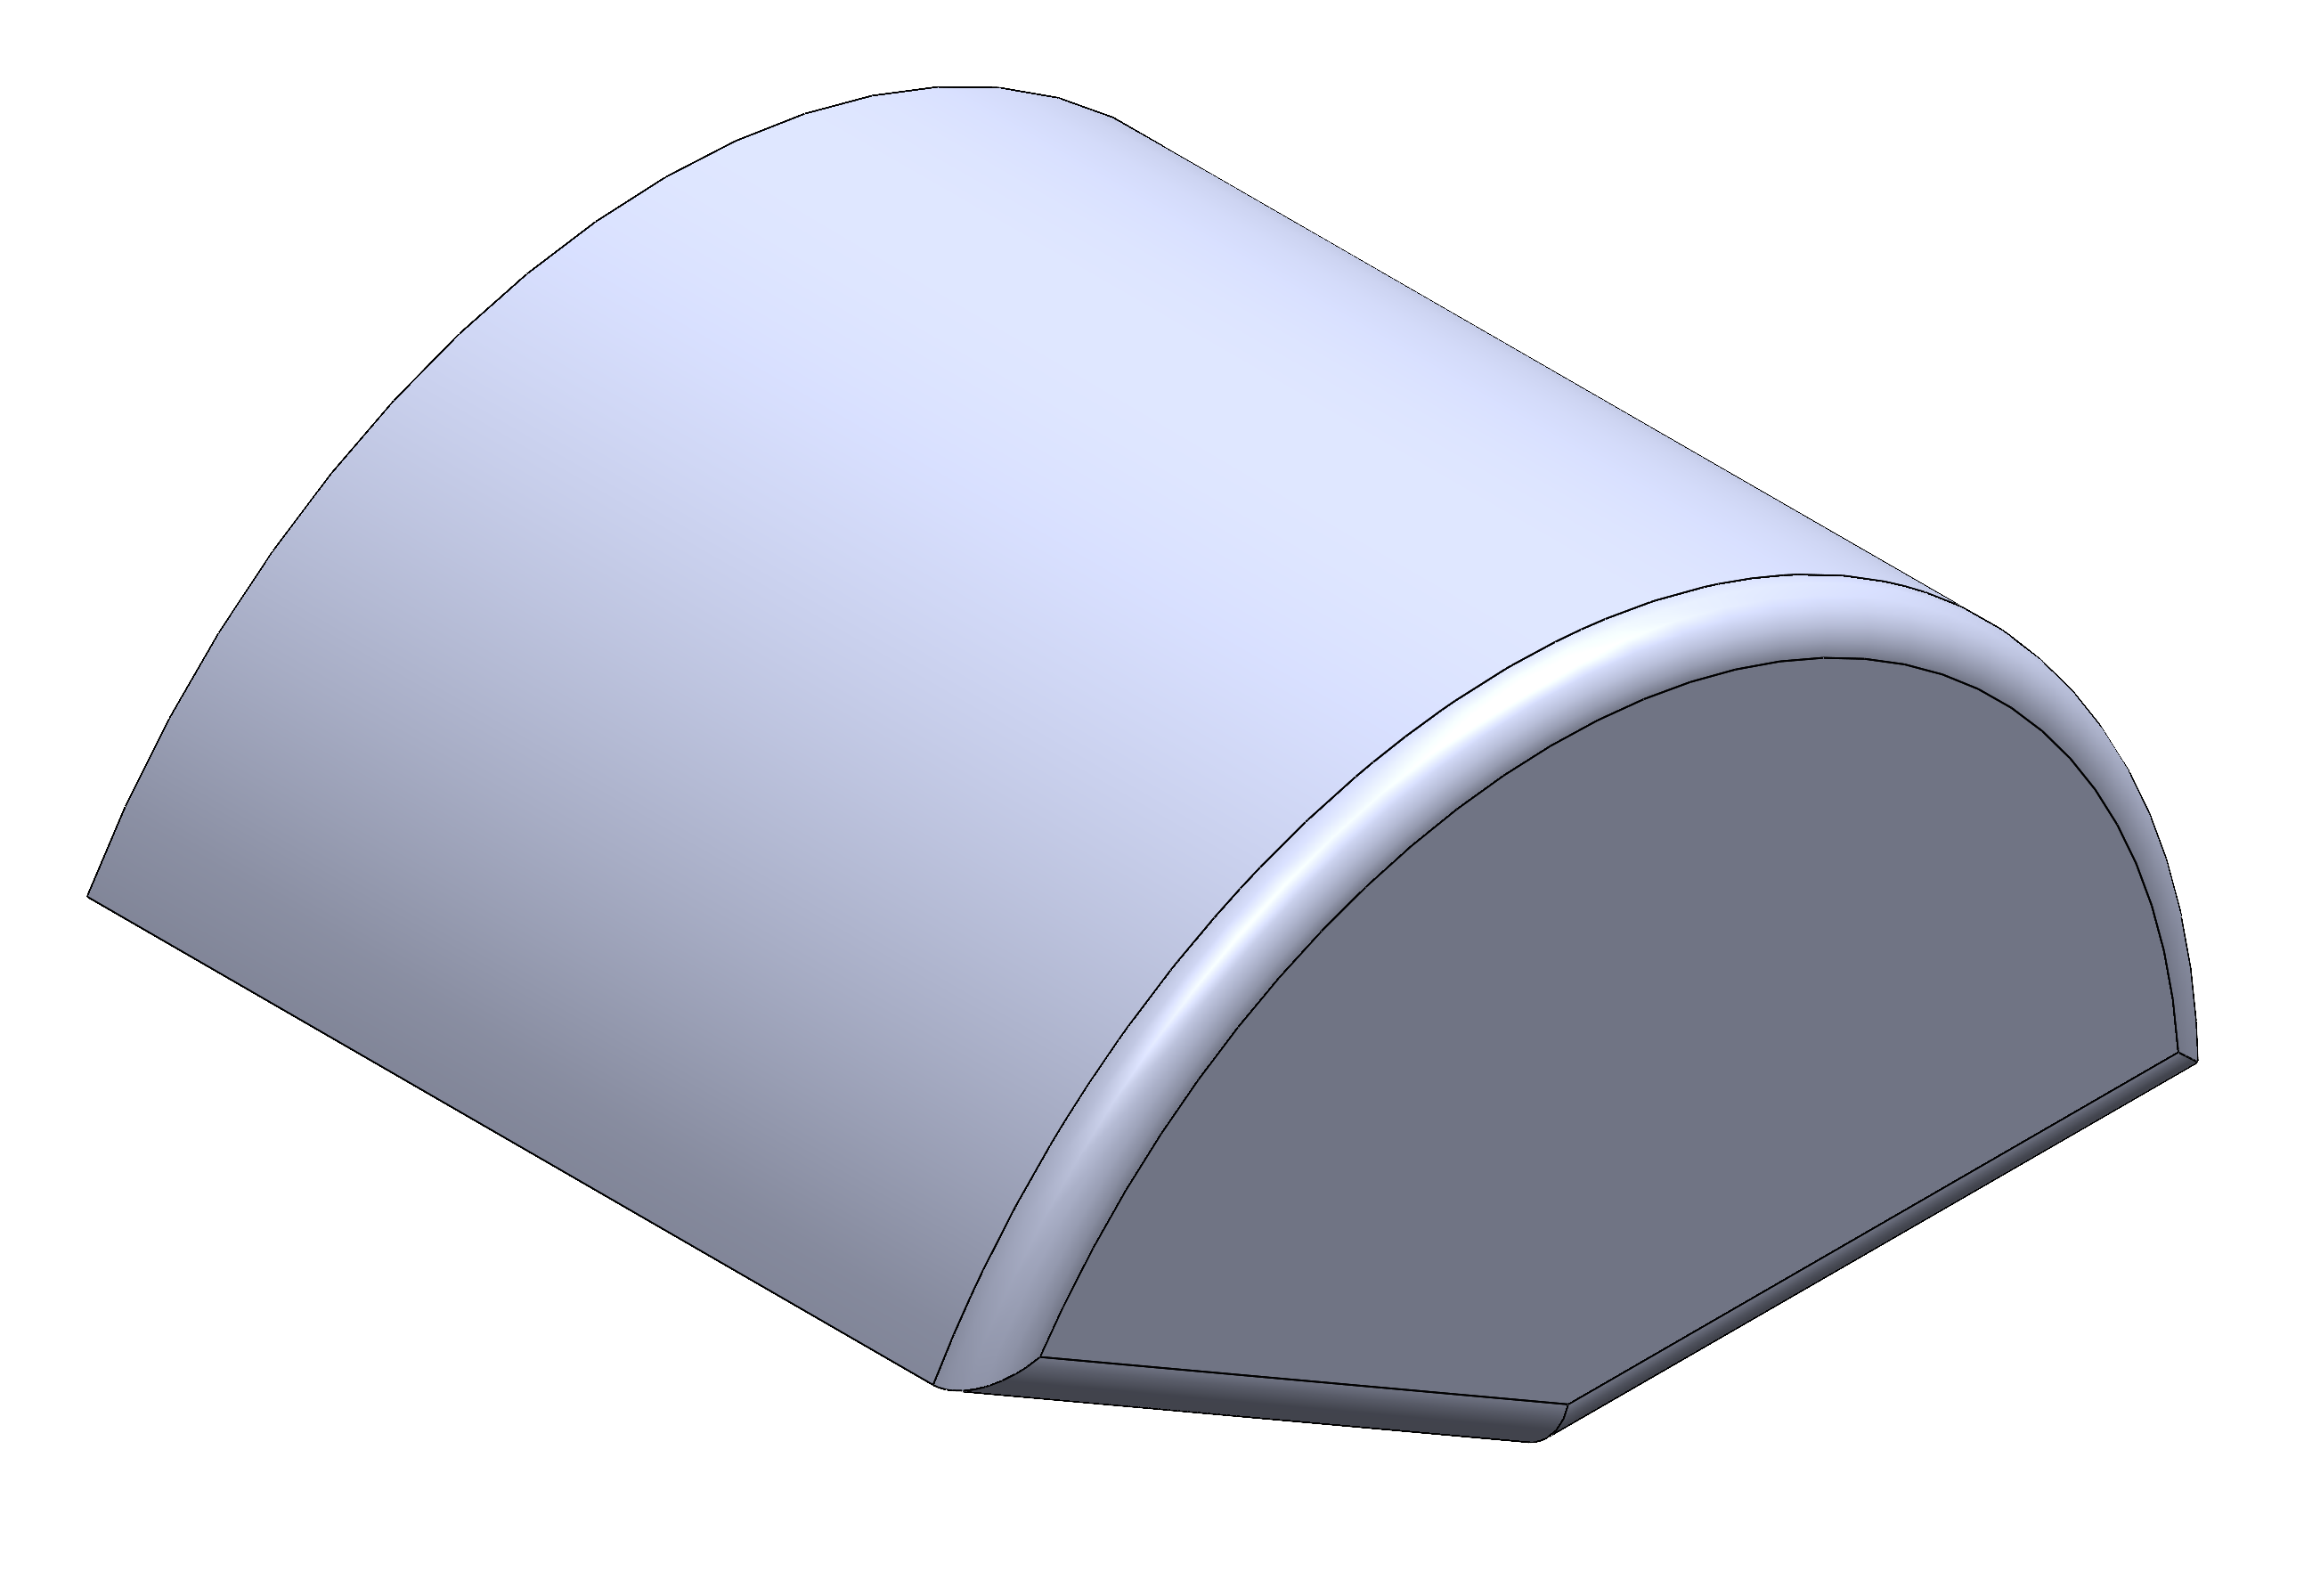
\includegraphics[width=\linewidth]{figures/parts/angle_curve.PNG}
        \scriptsize Angle Curve
      \end{minipage} &
      \begin{minipage}{0.3\linewidth}
        \centering
        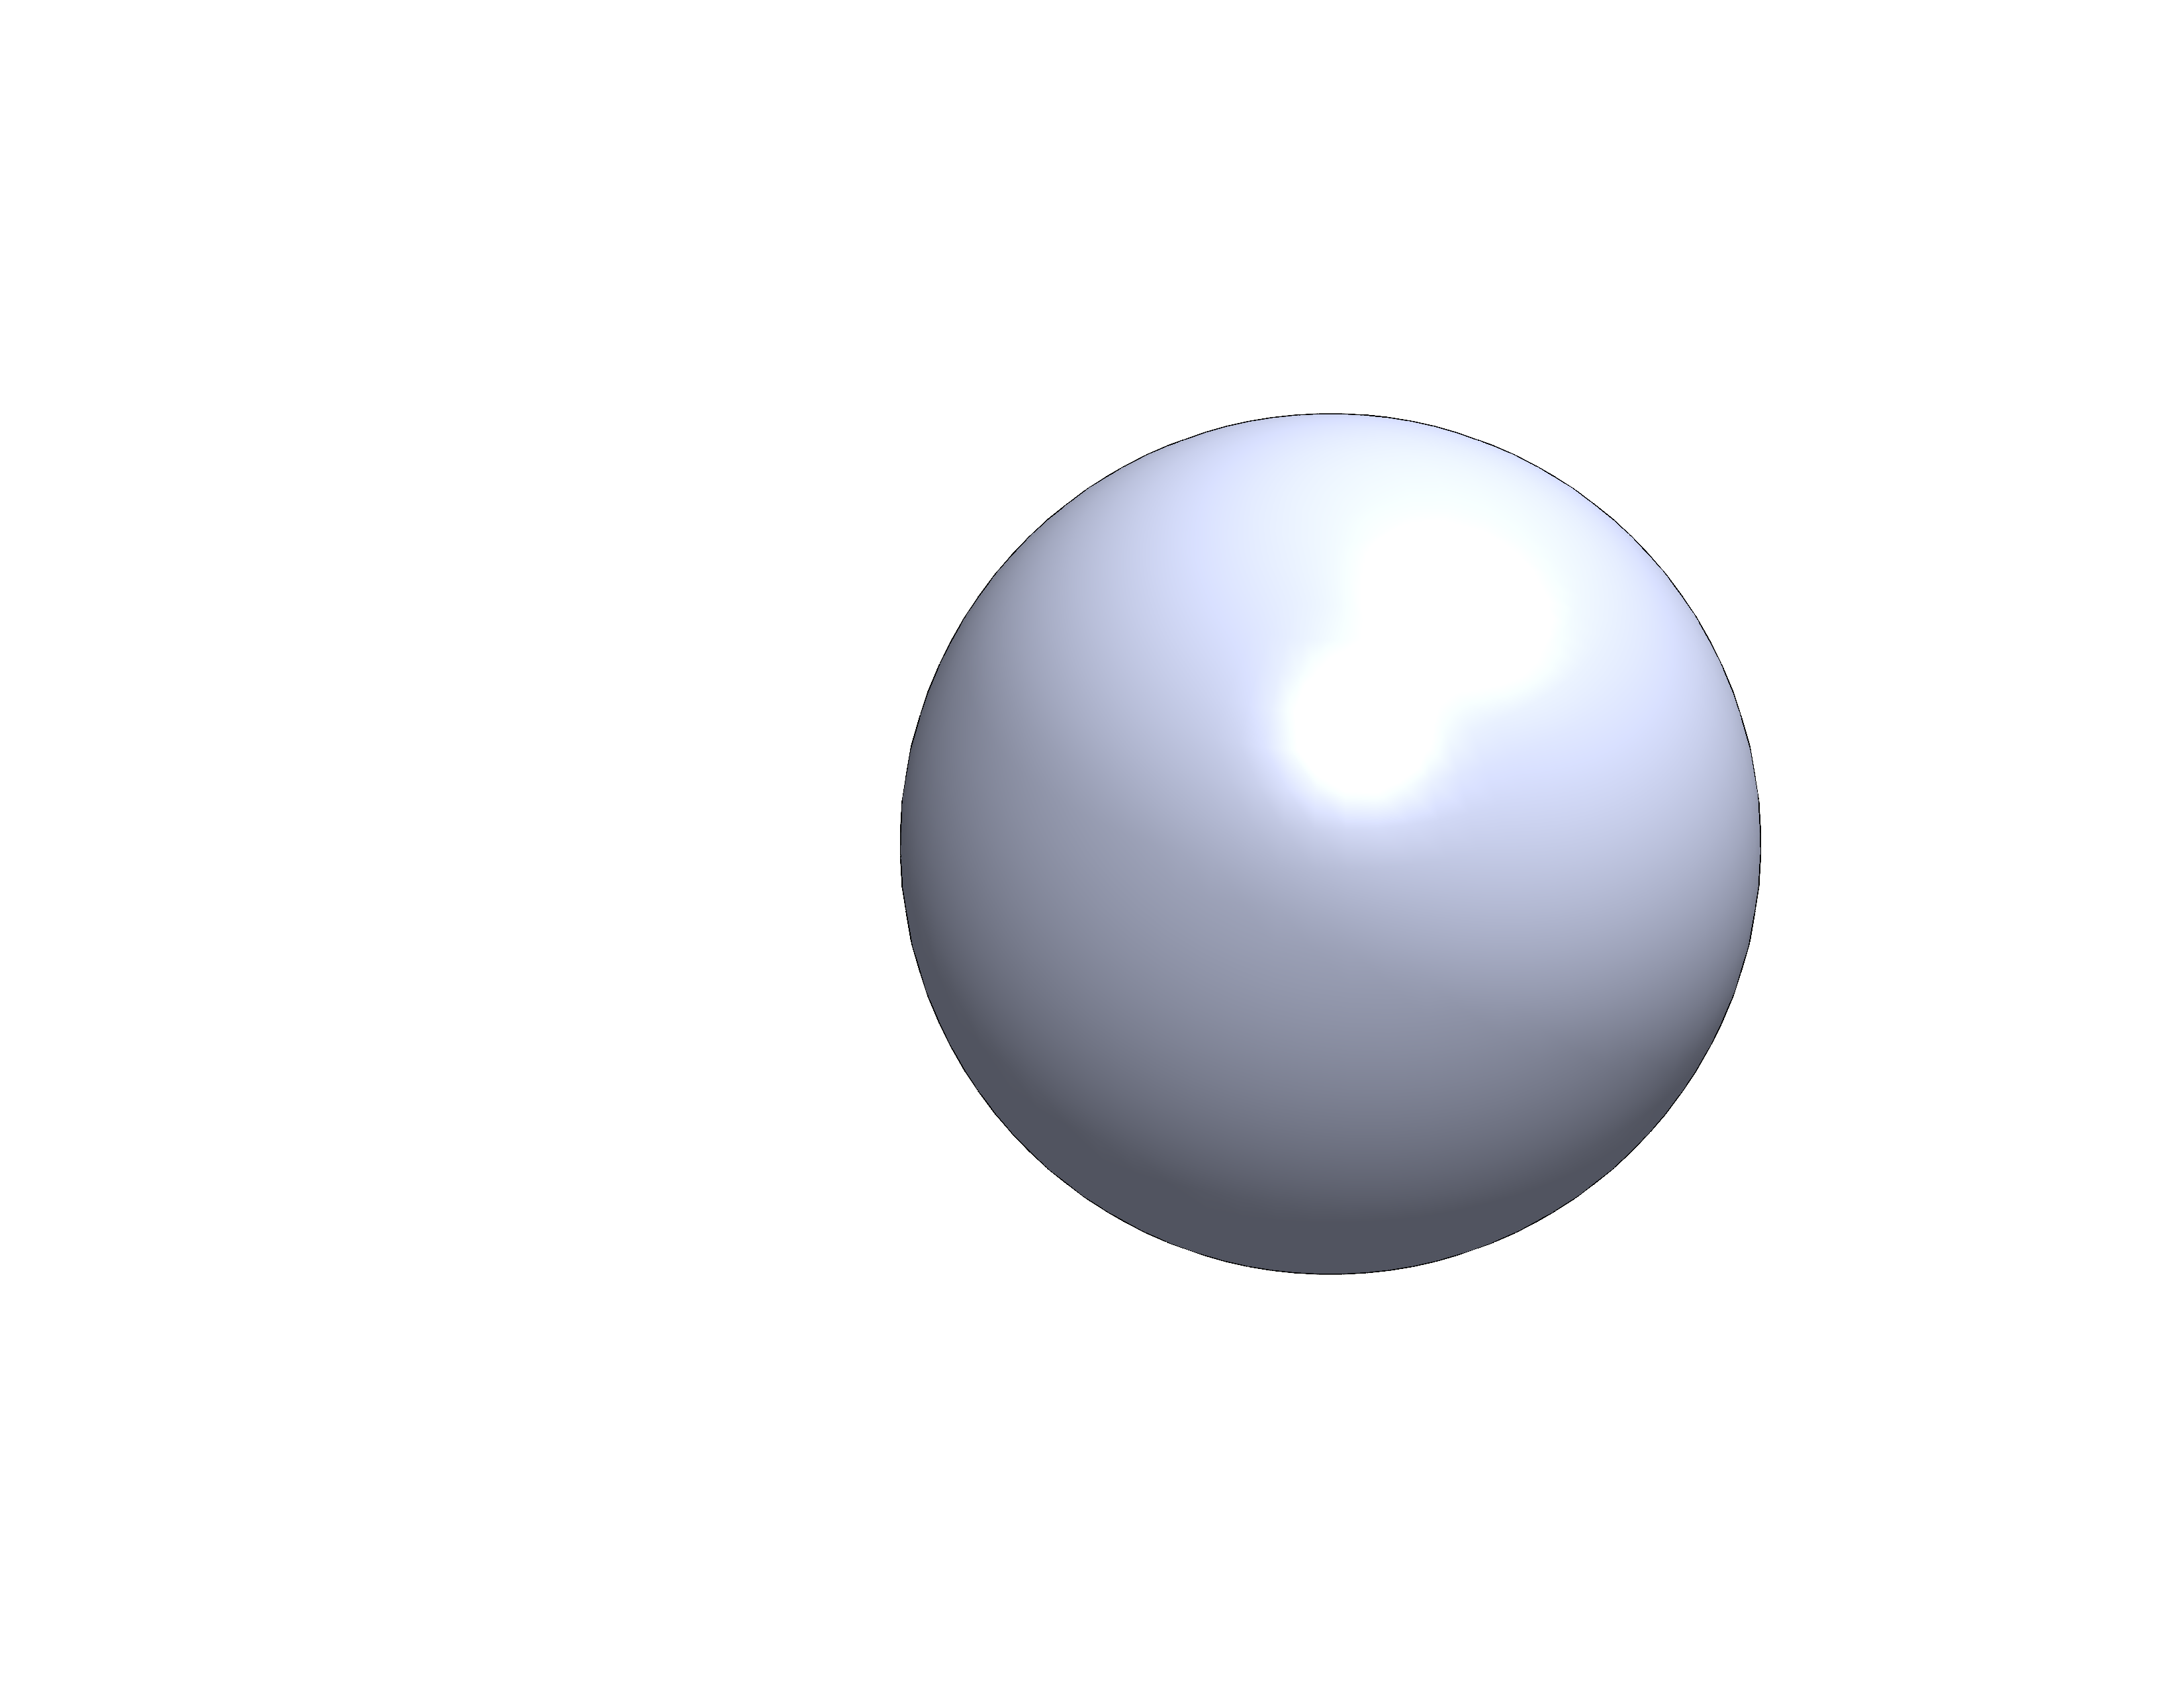
\includegraphics[width=\linewidth]{figures/parts/Ball.PNG}
        \scriptsize     Ball
      \end{minipage} &
      \begin{minipage}{0.3\linewidth}
        \centering
        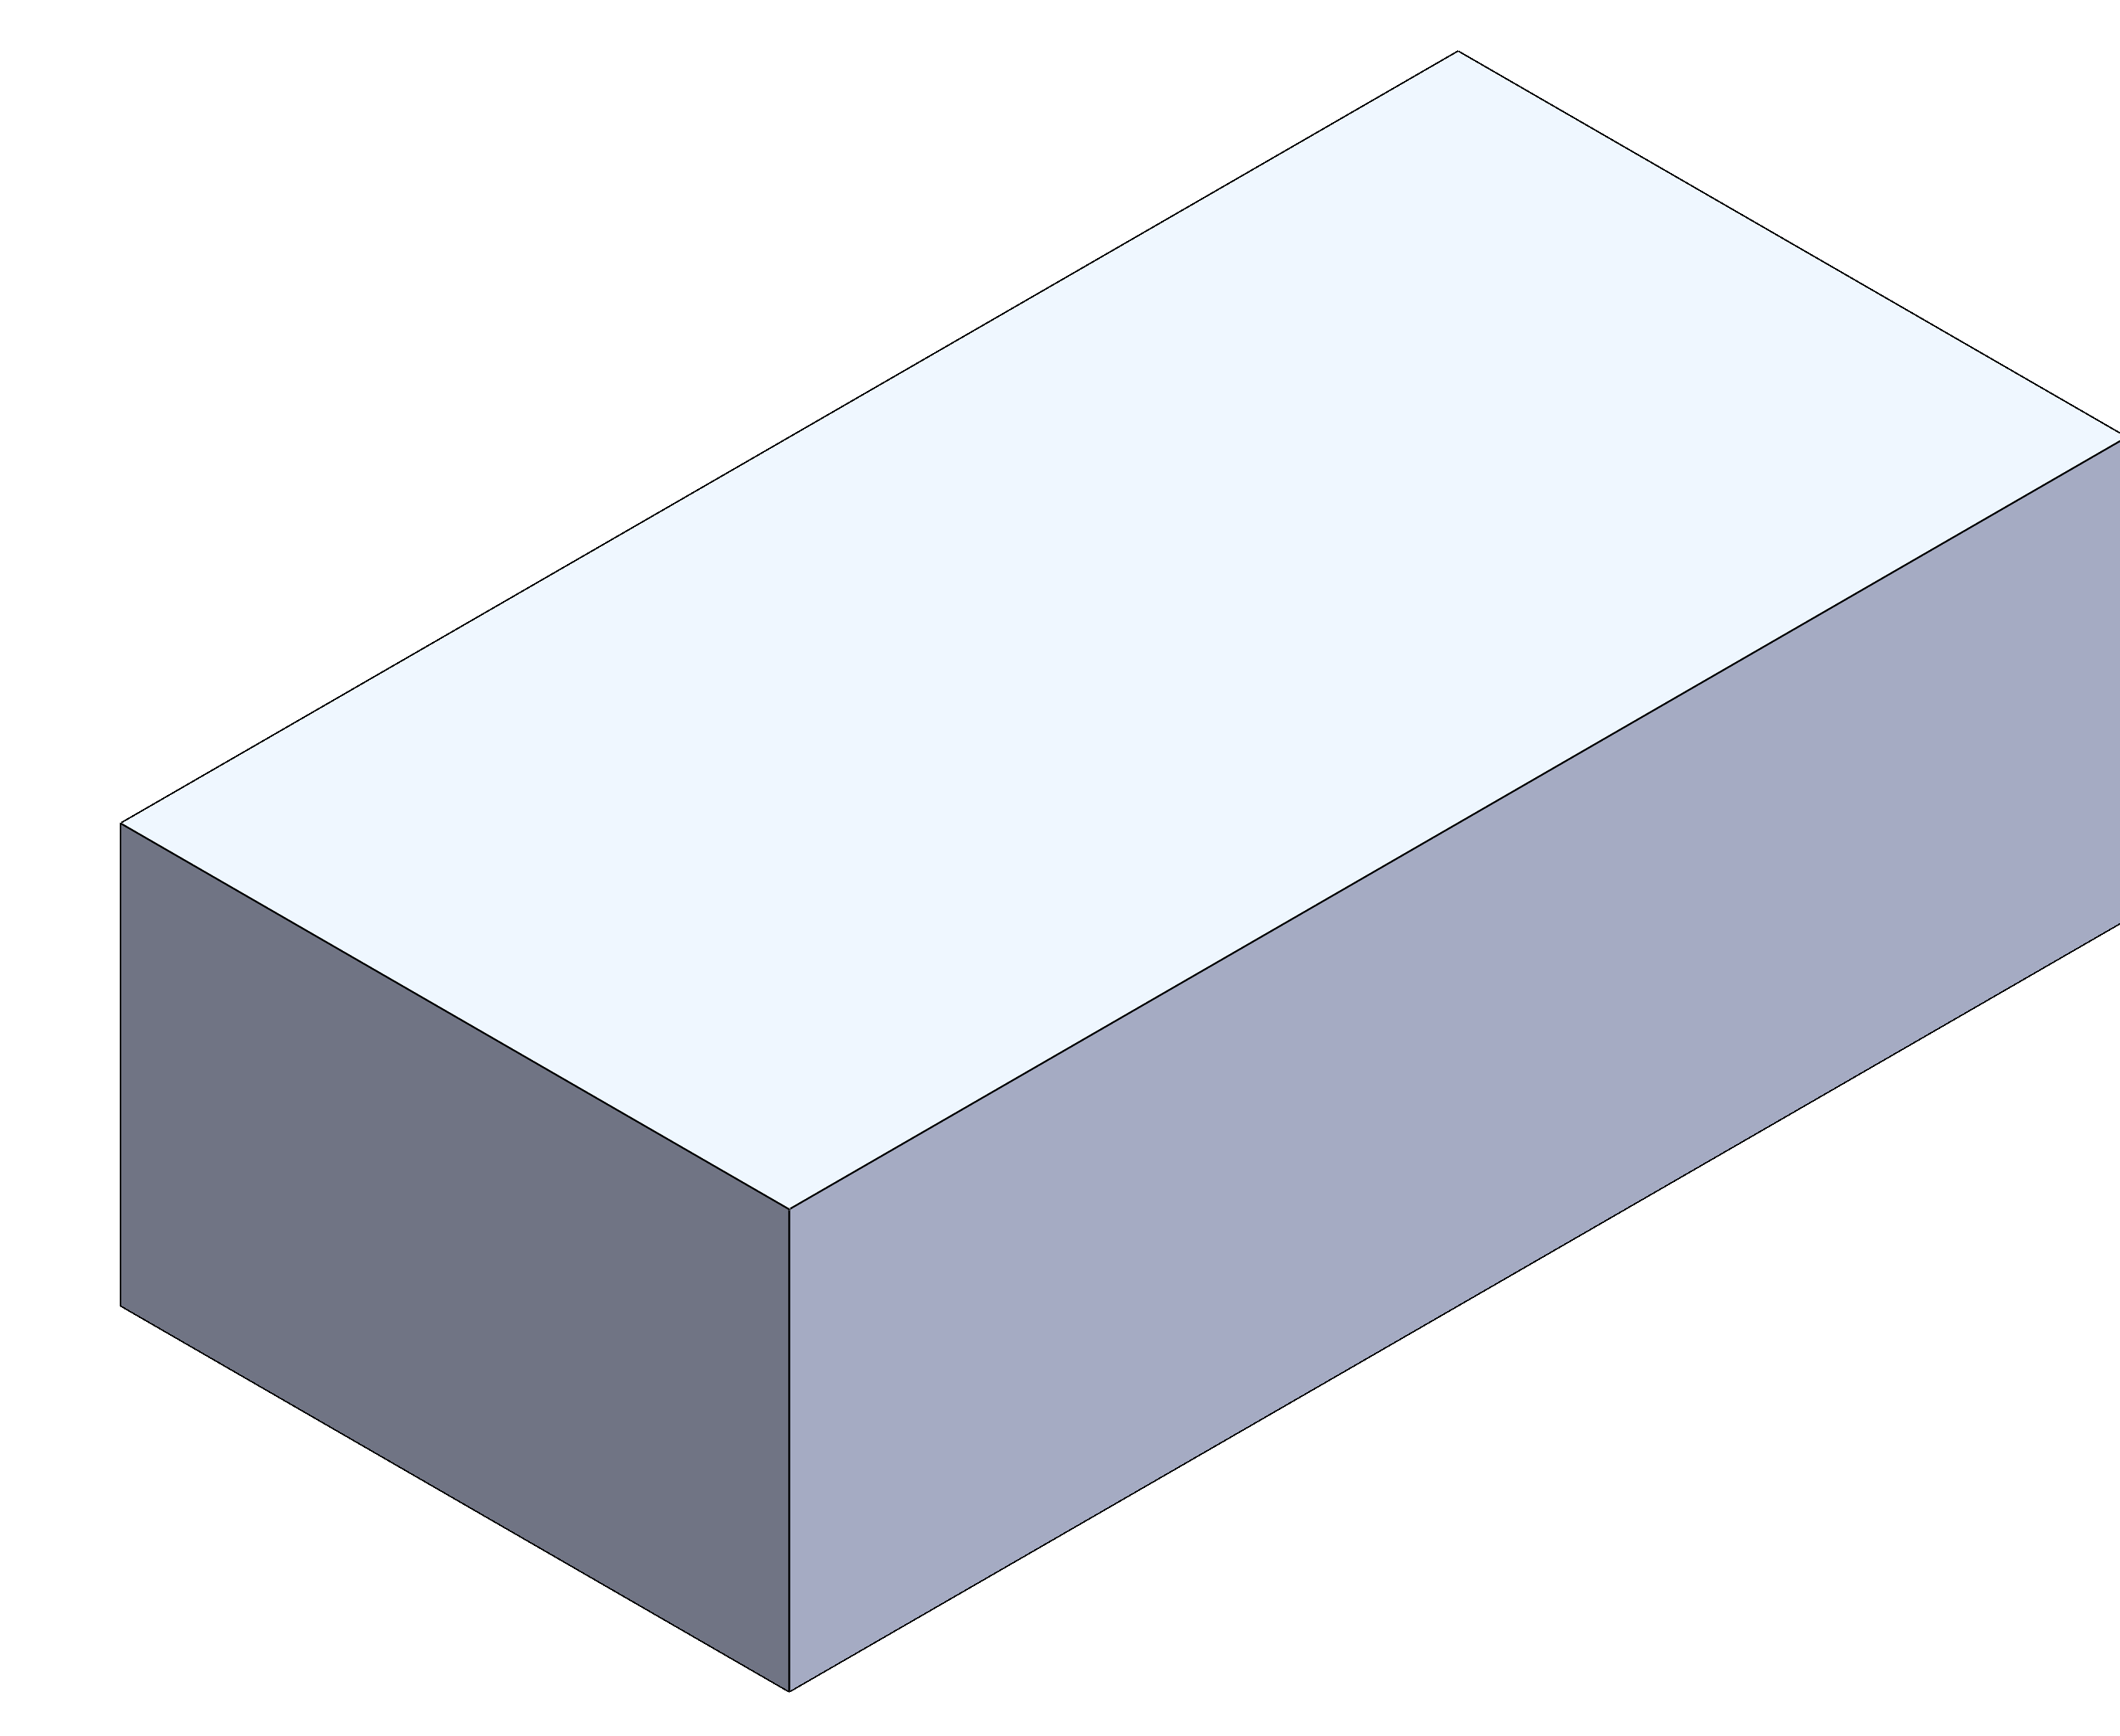
\includegraphics[width=\linewidth]{figures/parts/Box.PNG}
        \scriptsize Box
      \end{minipage} \\

      \begin{minipage}{0.3\linewidth}
        \centering
        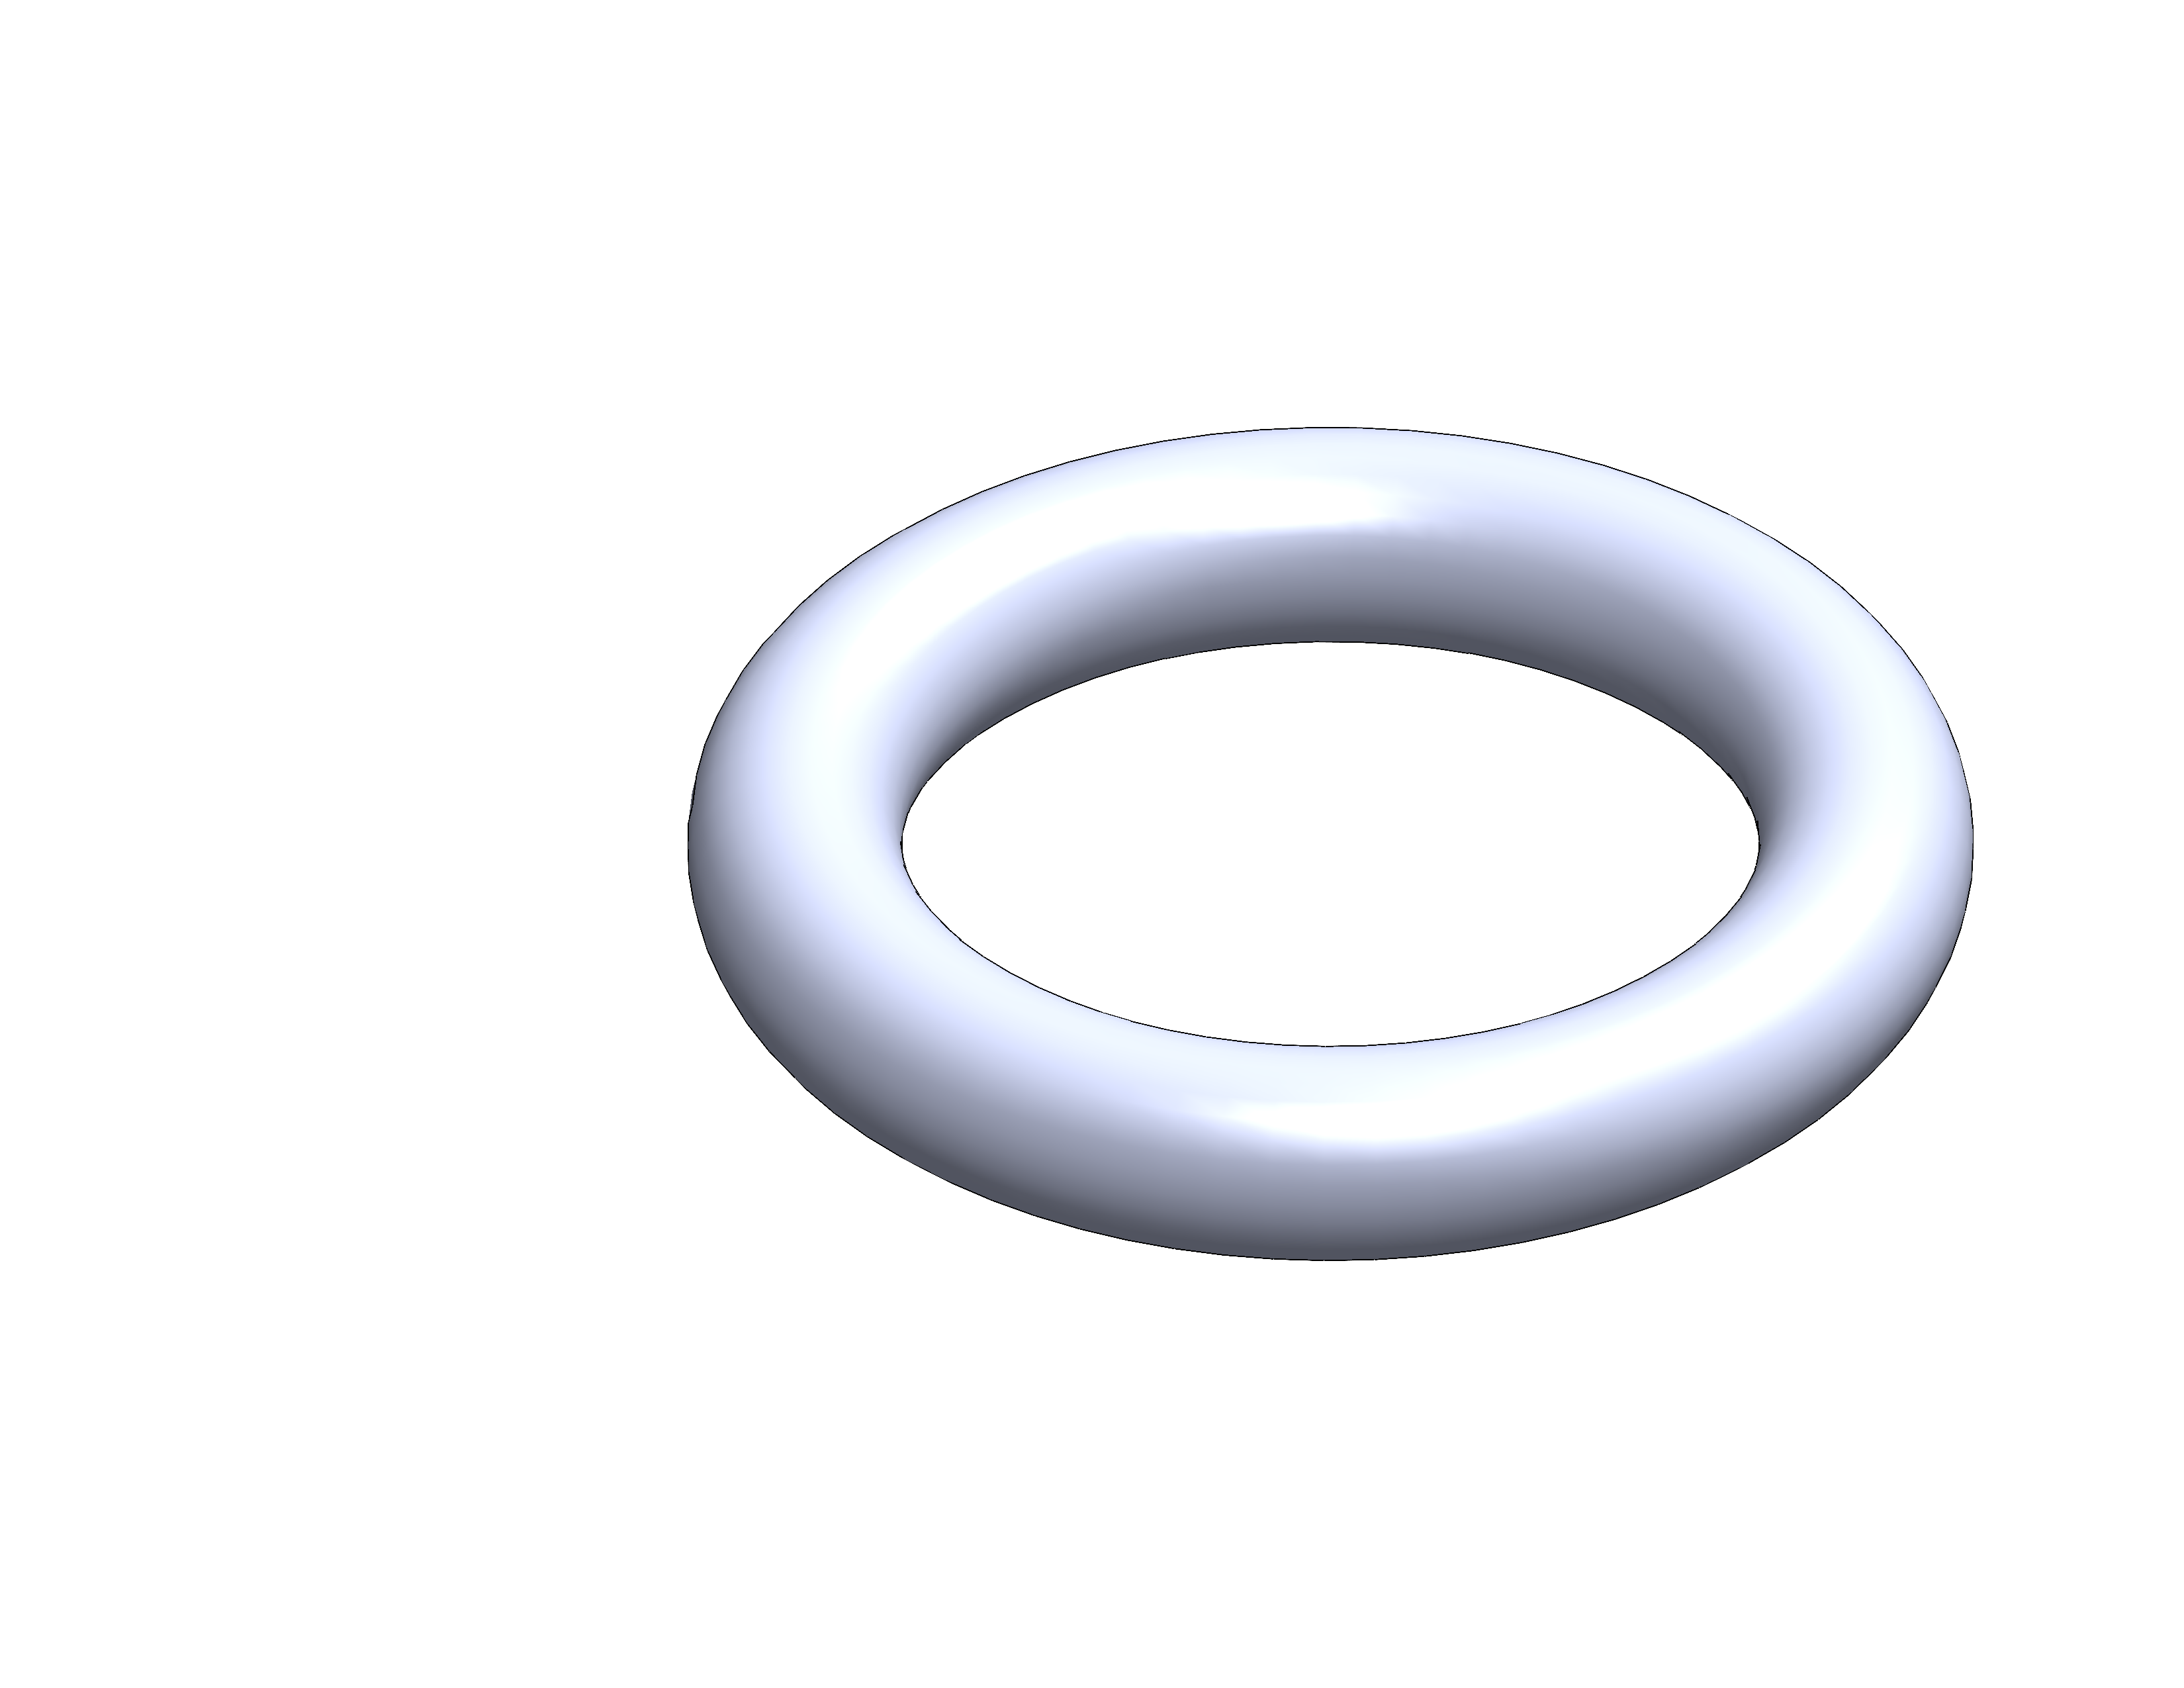
\includegraphics[width=\linewidth]{figures/parts/donut.PNG}
        \scriptsize Donut
      \end{minipage} &
      \begin{minipage}{0.3\linewidth}
        \centering
        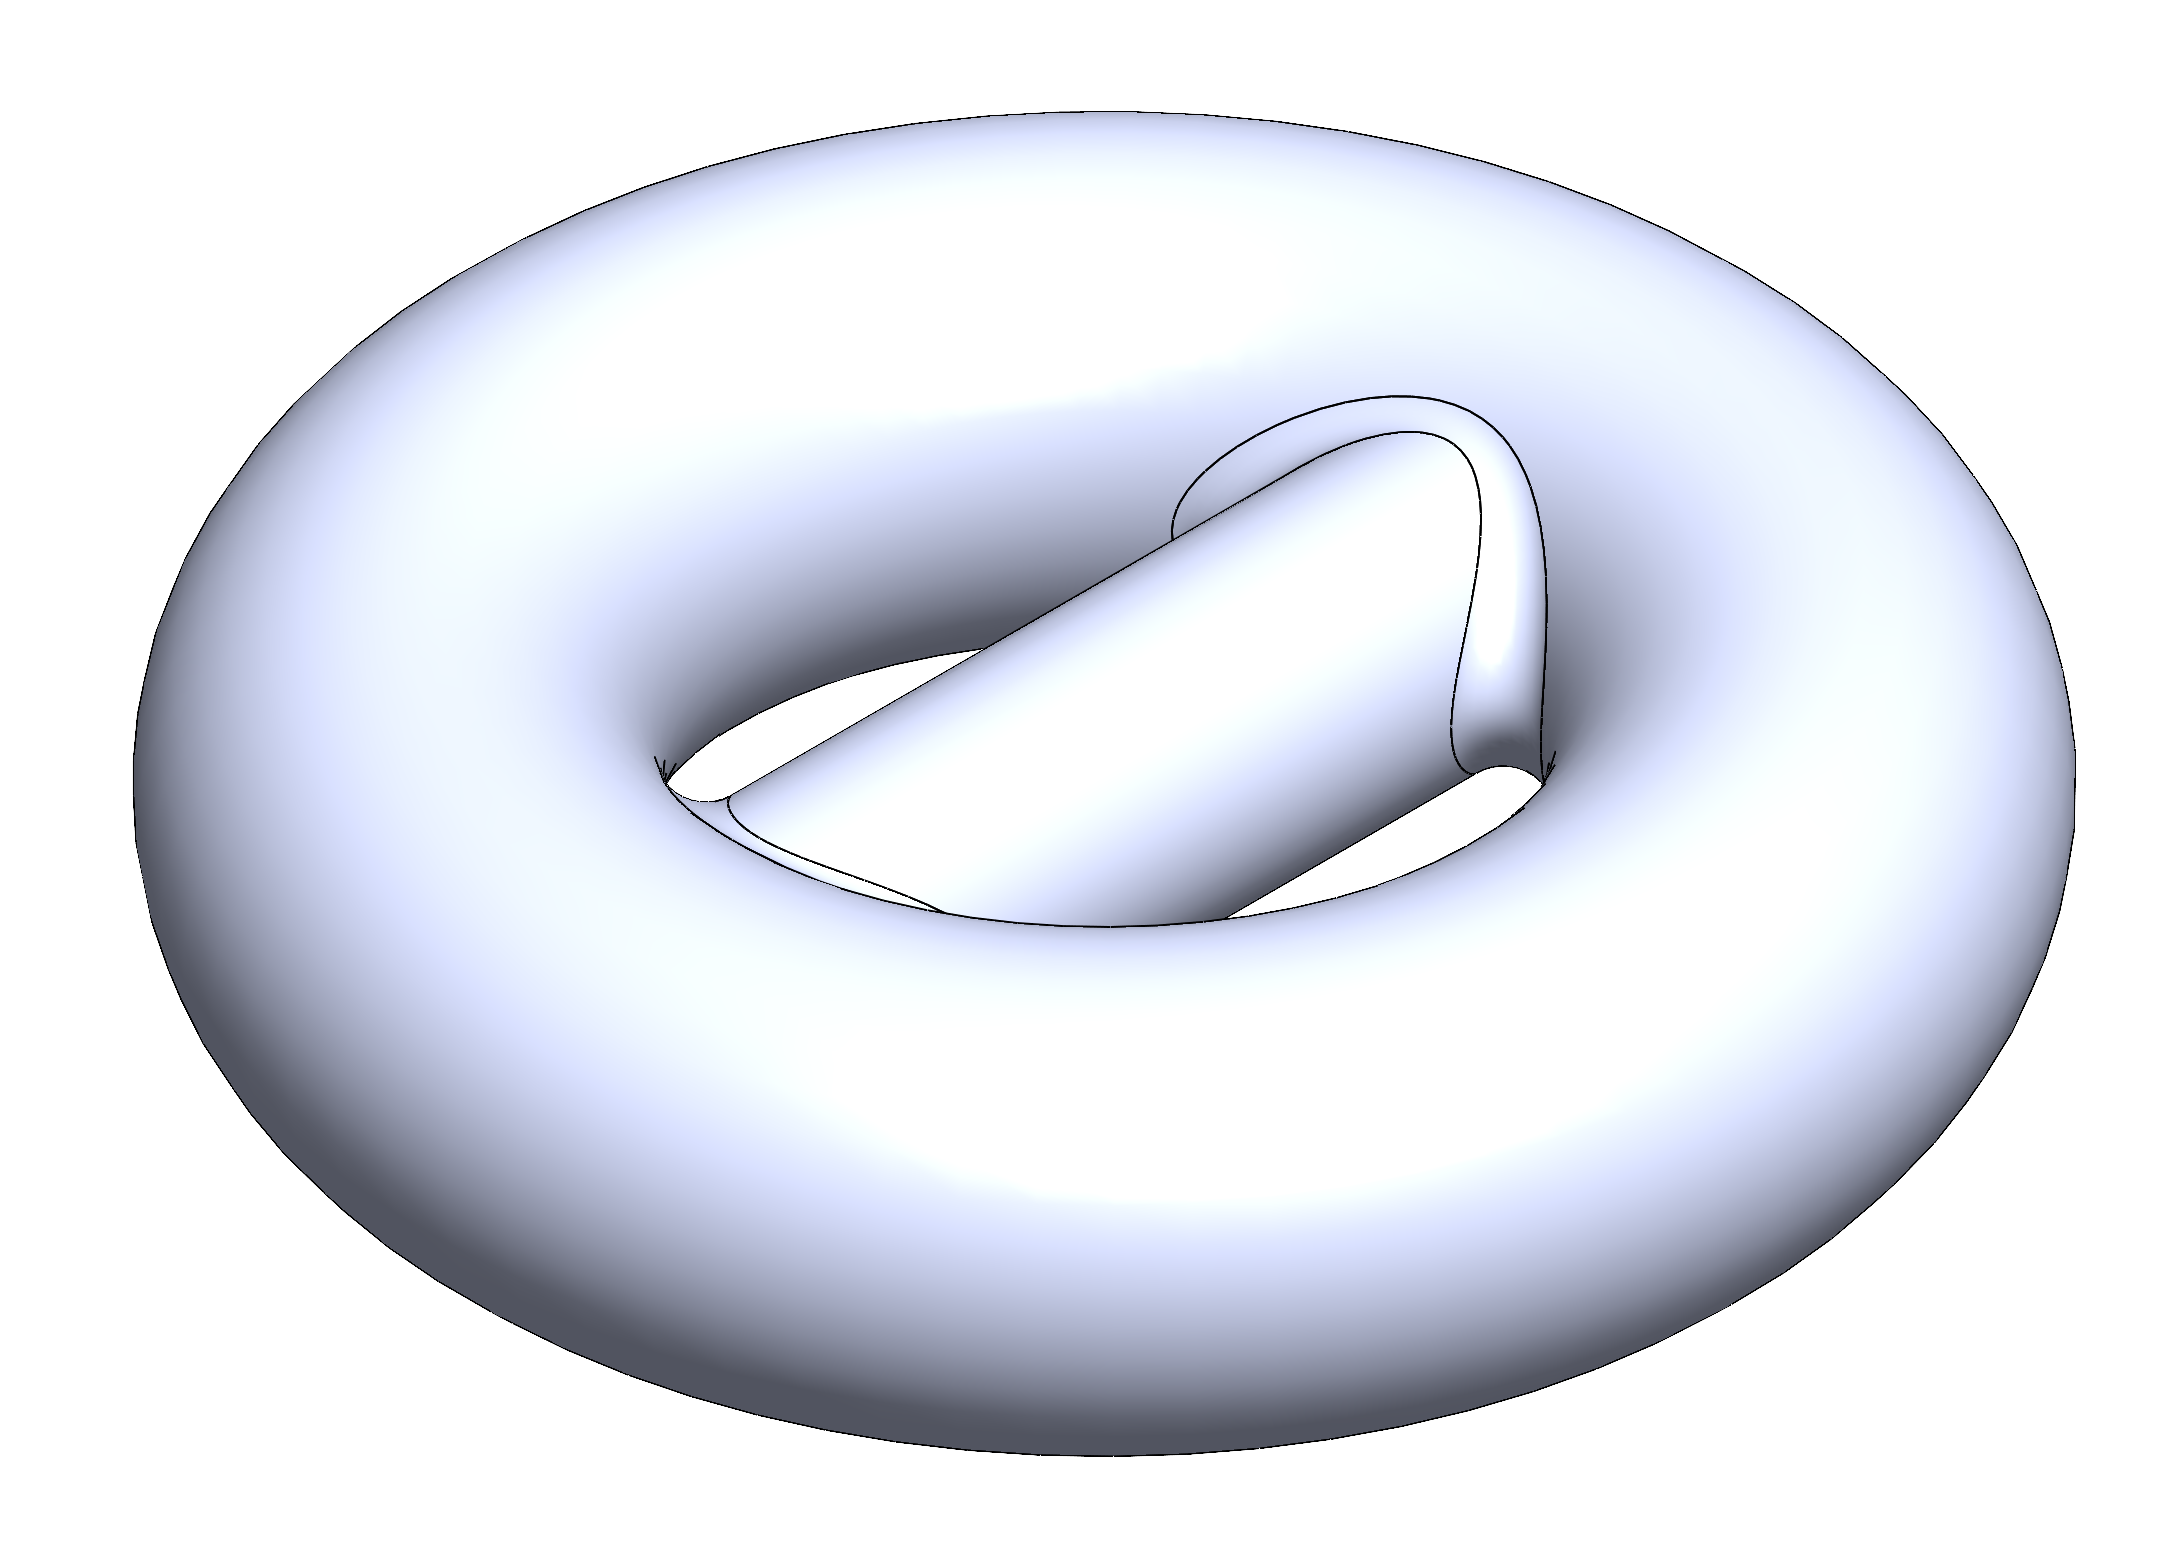
\includegraphics[width=\linewidth]{figures/parts/Donut_w_center.PNG}
        \scriptsize Donut w/ Center
      \end{minipage} &
      \begin{minipage}{0.3\linewidth}
        \centering
        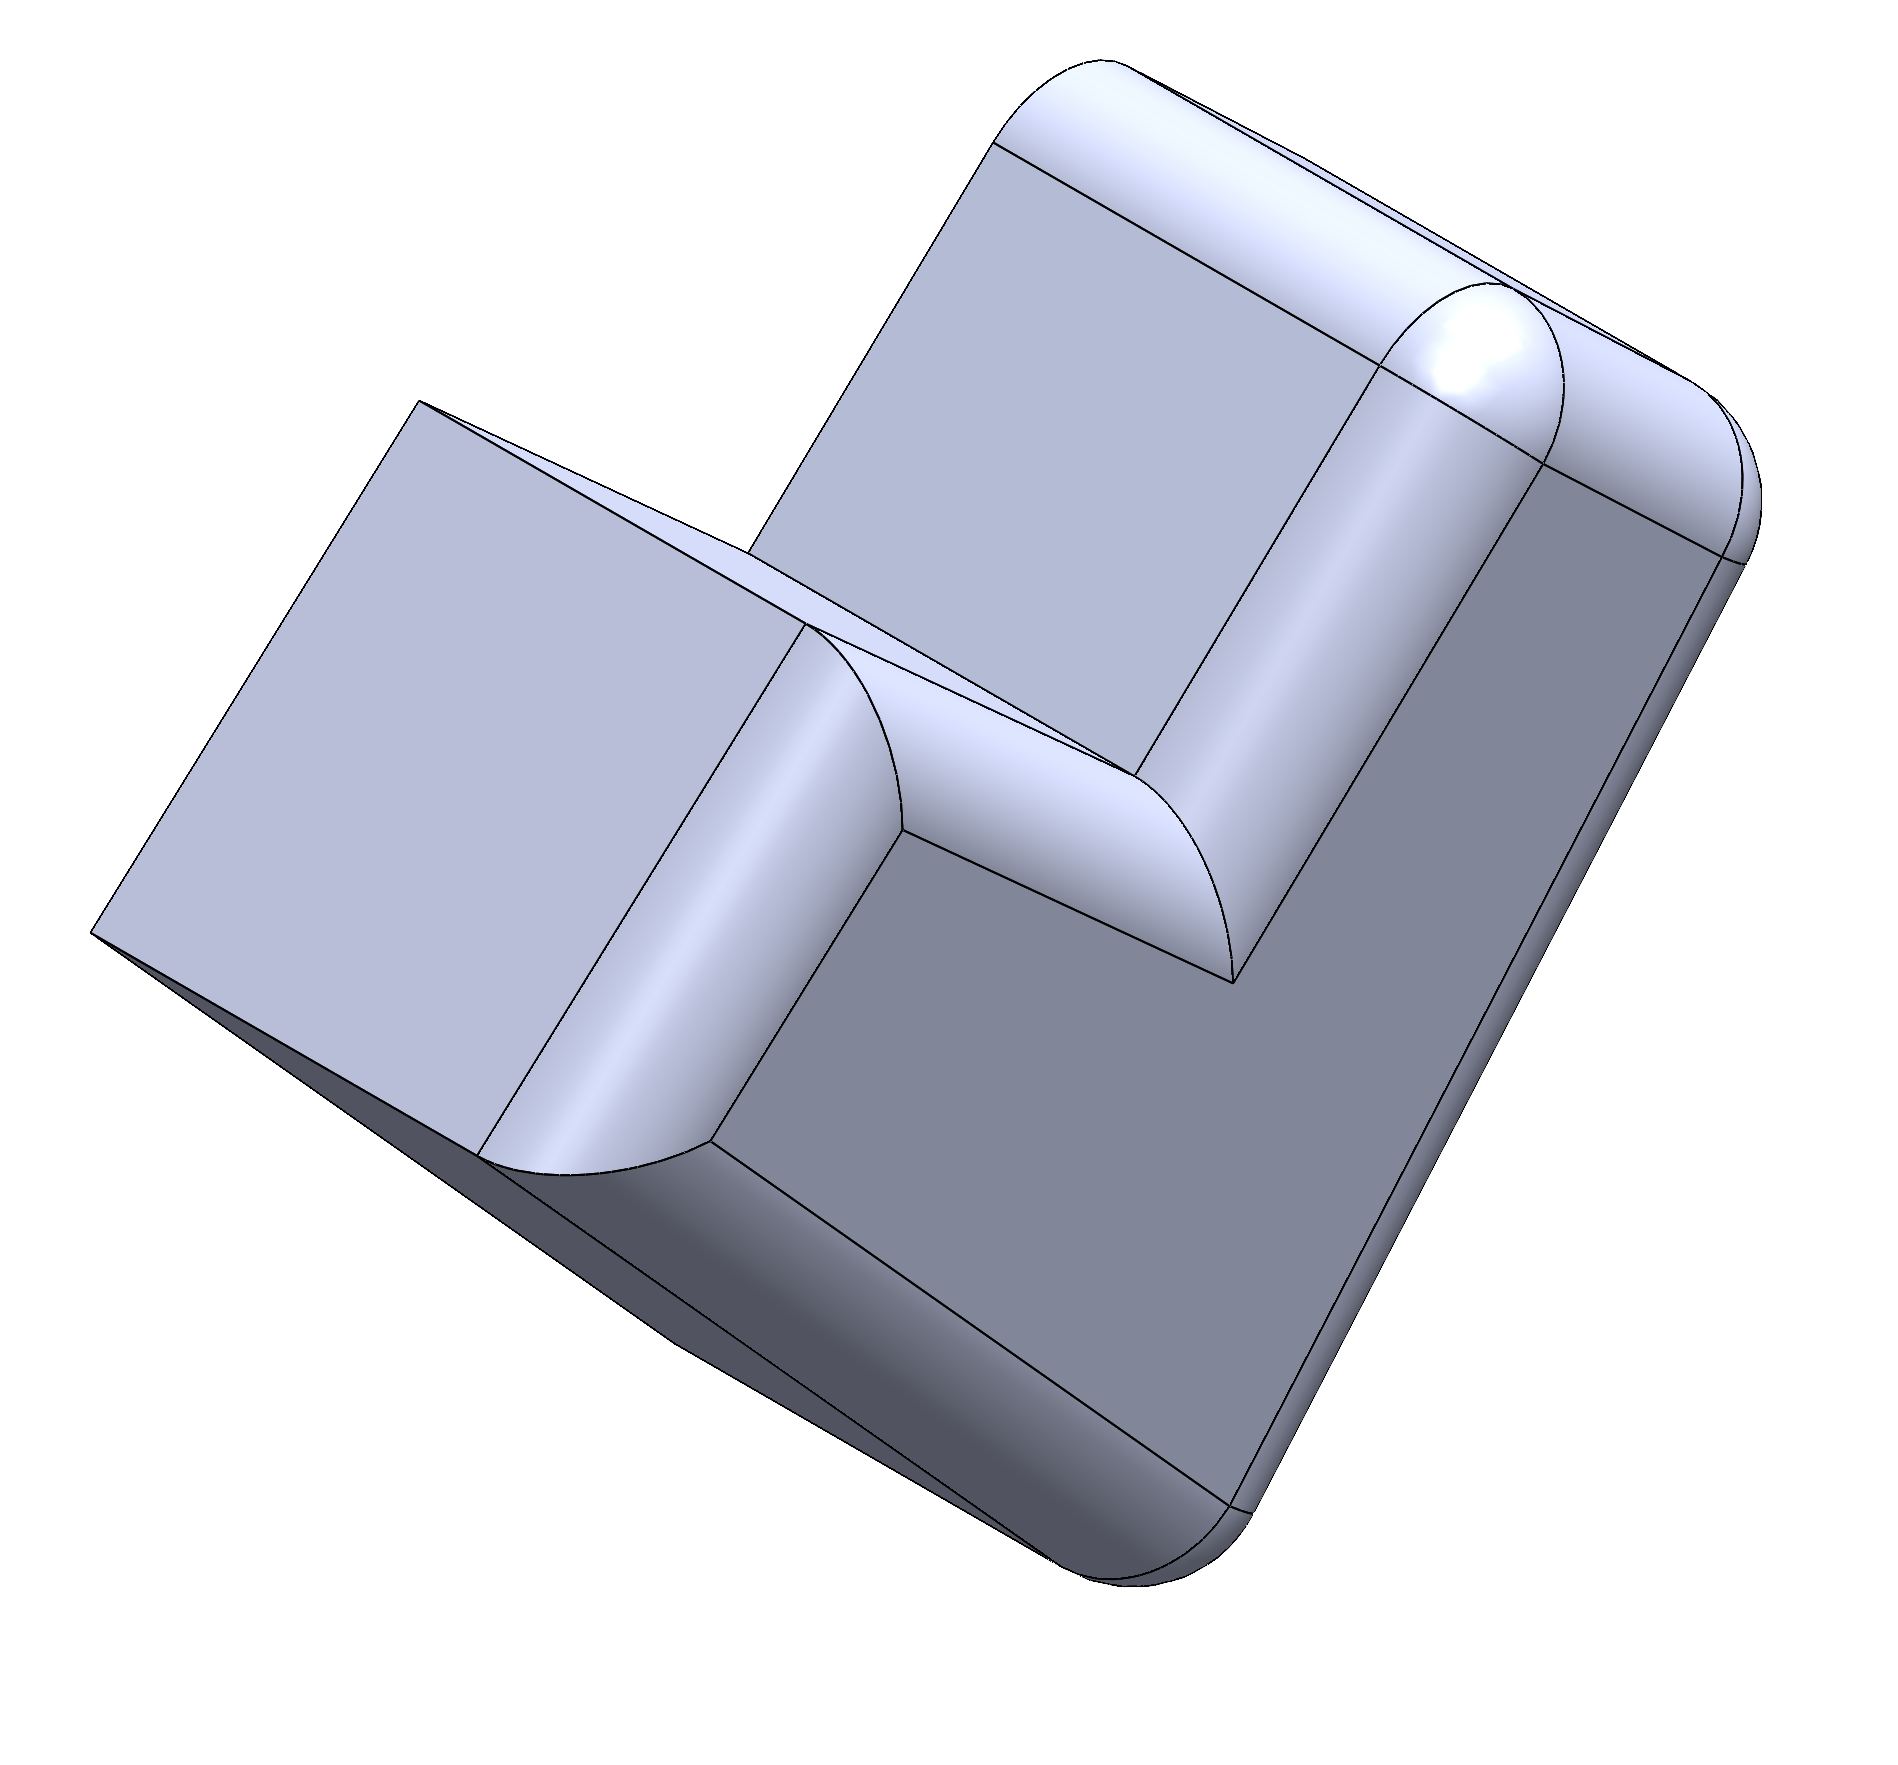
\includegraphics[width=\linewidth]{figures/parts/heart.PNG}
        \scriptsize Heart
      \end{minipage} \\

      \begin{minipage}{0.3\linewidth}
        \centering
        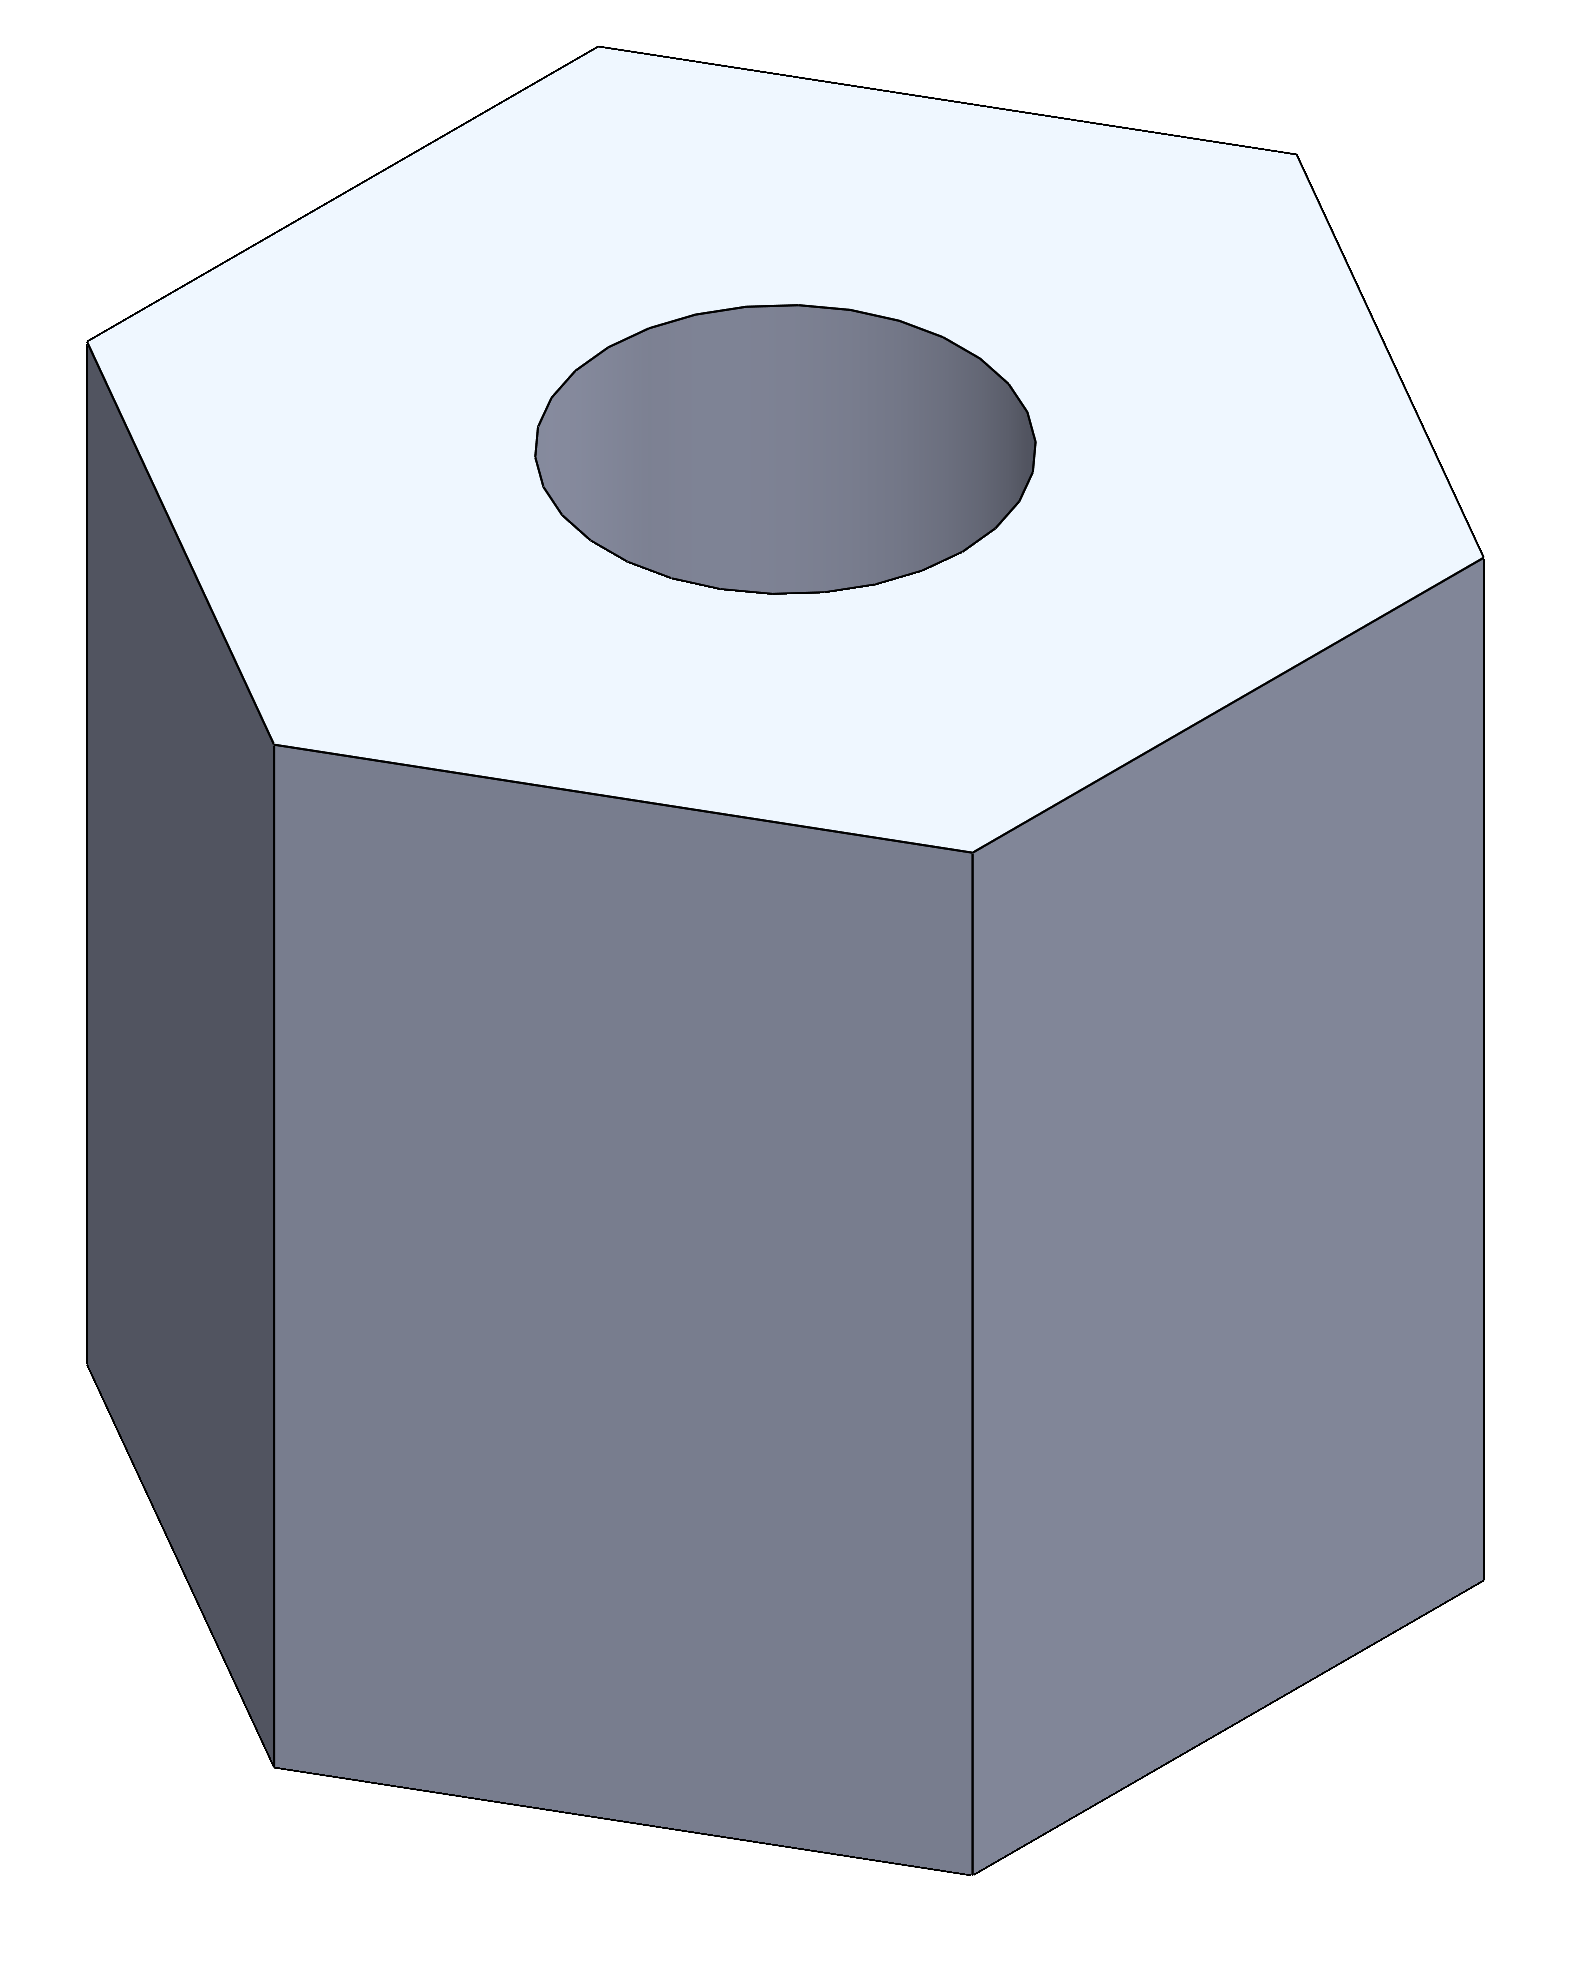
\includegraphics[width=\linewidth]{figures/parts/nut.PNG}
        \scriptsize Nut
      \end{minipage} &
      \begin{minipage}{0.3\linewidth}
        \centering
        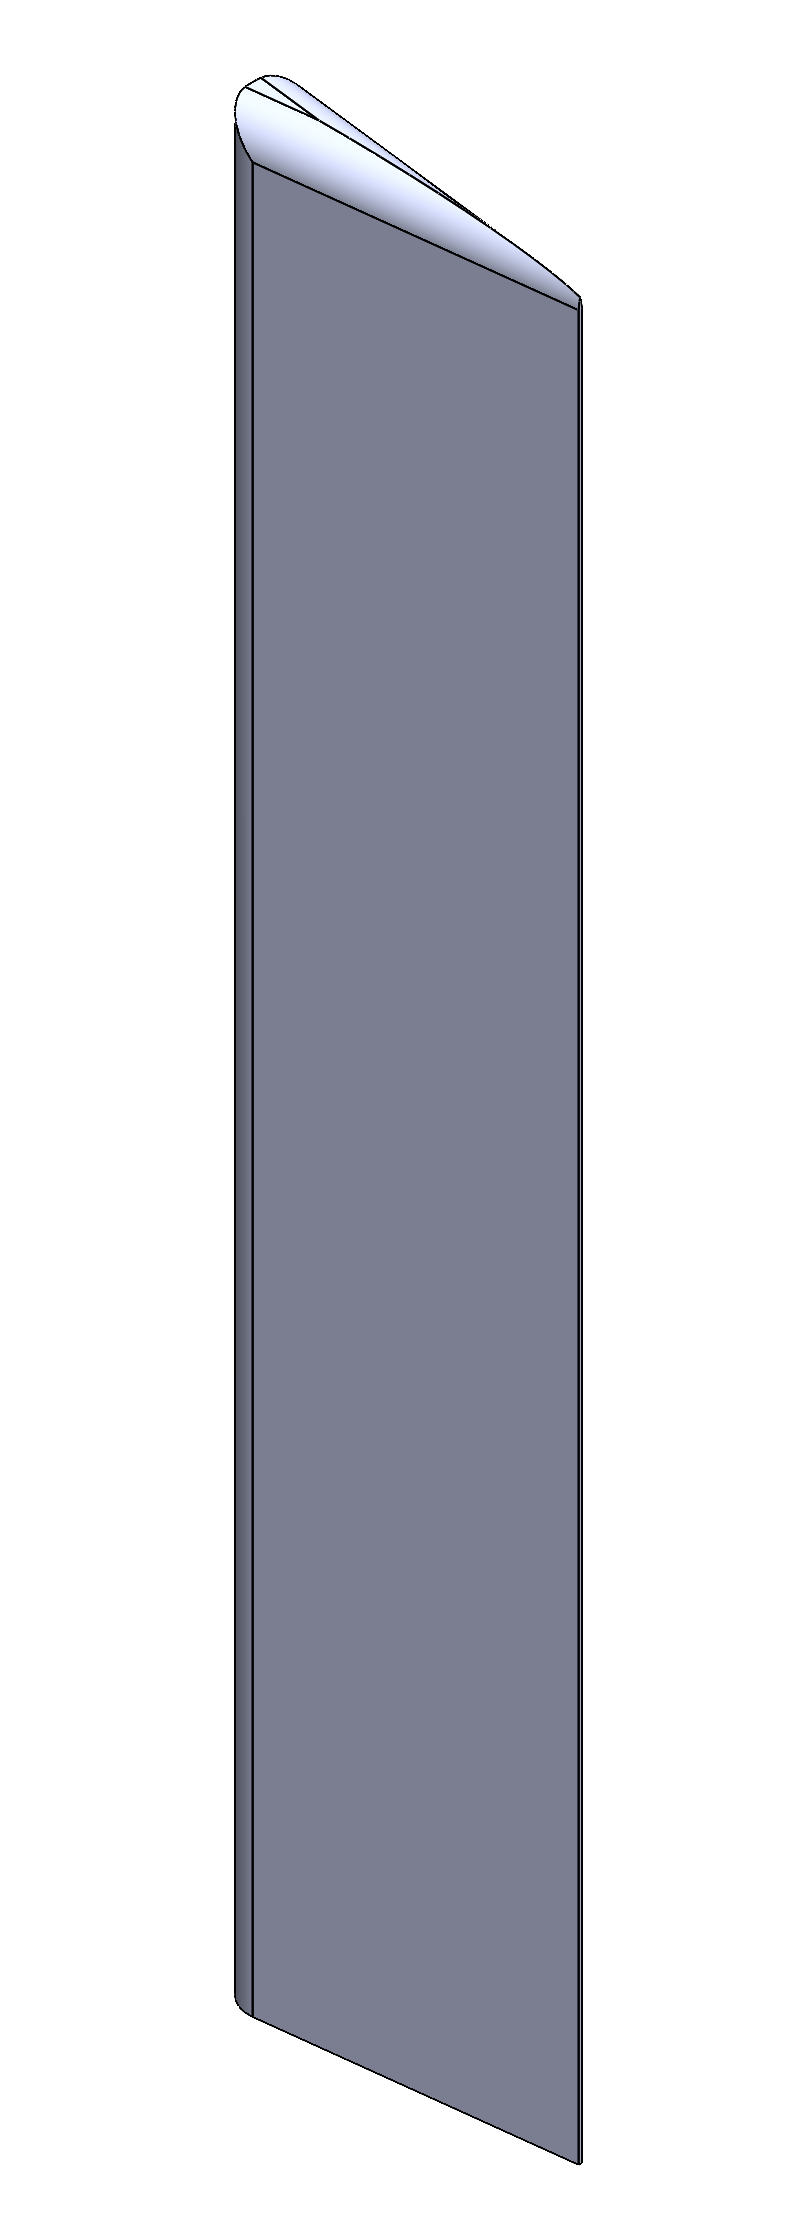
\includegraphics[width=\linewidth]{figures/parts/wedge.PNG}
        \scriptsize Wedge
      \end{minipage} &
      % Last column left blank
      \begin{minipage}{0.3\linewidth} \end{minipage} \\
    \end{tabular}
  \end{minipage}

  \caption{Shapes used in the dataset for MLP training.}
  \label{fig:part_shapes_grid}
\end{figure}















